Le groupe est composé de 5 membres. Chaque membre possède sa manière de travailler, de comprendre, de communiquer. Une des difficultés d’un travail d’équipe est de pouvoir combiner tous ces caractères pour que le projet se déroule dans les meilleures conditions et que chacun puisse trouver sa place. Donc pour comprendre le fonctionnement de chacun, chaque membre a dû présenter ses points forts et ses points faibles. Le but de cette démarche est de pouvoir répartir les tâches au mieux tout en privilégiant le transfert de compétences. Ceci a été fait par exemple lors de la présentation orale formative de mi-parcours, où les membres qui se sentaient le moins à l’aise dans l'exercice ont choisi de faire cette présentation afin de pouvoir profiter de l'opportunité.

\subsubsection{Organisation et communication}

La répartition des tâches se fait spontanément en fonction des besoins pour l’avancée du projet ainsi que des membres qui ont travaillé sur des tâches similaires dans le passé. Ceci offre l’avantage d’une meilleure gestion du temps lors des réunions car les membres sont au courant des problèmes à régler. Cependant un diagramme de Gantt (cf. annexe) a été créé pour aussi avoir une vision plus globale de l’avancement du projet et également se fixer des dates butoir.

A côté des moyens de communication habituellement utilisés tels que l'utilisation de mails et de réseau sociaux, des outils plus spécifiques ont été mis en place afin d'améliorer l'implication des membres et l'efficacité du travail collectif. Tout d'abord, un dépôt git a été créé \footnote{\url{https://github.com/nathdwek/projetBa2} et \url{https://github.com/nathdwek/rapportProjetBa2}} afin de pouvoir profiter de tous les avantages qu'offre un contrôleur de version distribué: sécurité, travail simultané sur plusieurs aspects du code tout en maintenant une version parfaitement fonctionelle, possibilité de consulter l'historique,~\ldots Nous avons essayé de passer systématiquement par l'usage de branches afin de nouveau de gagner en sécurité, ce qui permet à n'importe quel membre d'essayer sans crainte et sans perte de temps d'implémenter une fonctionnalité ou de corriger une erreur éventuelle. D'autre part, nous avons utilisé Zotero pour la mise en commun, l'uniformisation et l'export en format Bibtex des ressources bibliographiques.

\begin{figure}[htb]
  \centering
  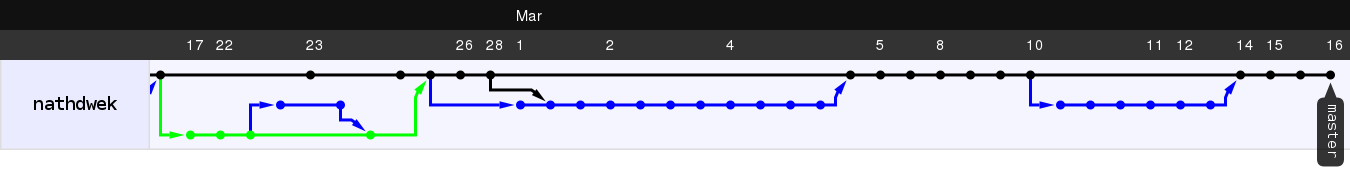
\includegraphics[width=\textwidth]{pics/workflow.png}
    \caption{Réseau de commits récents du projet}
\end{figure}
